% Created by tikzDevice version 0.12.6 on 2025-09-08 08:58:31
% !TEX encoding = UTF-8 Unicode
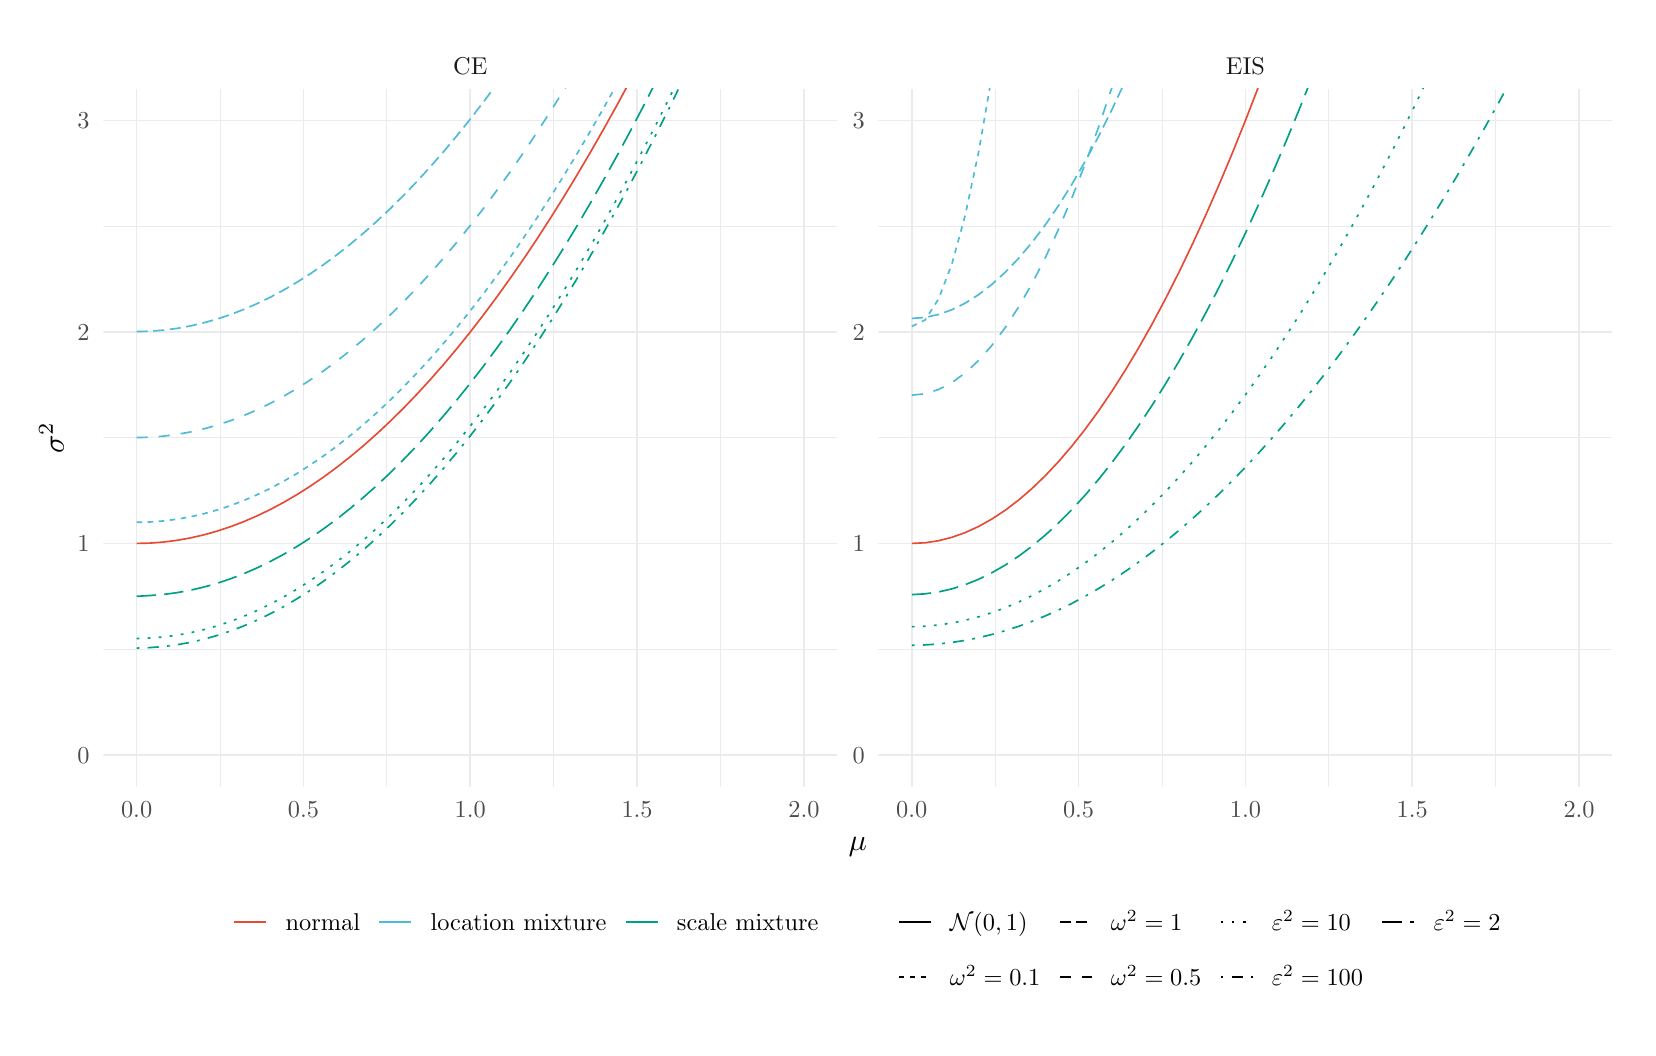
\begin{tikzpicture}[x=1pt,y=1pt]
\definecolor{fillColor}{RGB}{255,255,255}
\path[use as bounding box,fill=fillColor,fill opacity=0.00] (0,0) rectangle (578.16,361.35);
\begin{scope}
\path[clip] ( 27.31, 87.09) rectangle (292.56,339.28);
\definecolor{drawColor}{gray}{0.92}

\path[draw=drawColor,line width= 0.3pt,line join=round] ( 27.31,136.77) --
	(292.56,136.77);

\path[draw=drawColor,line width= 0.3pt,line join=round] ( 27.31,213.19) --
	(292.56,213.19);

\path[draw=drawColor,line width= 0.3pt,line join=round] ( 27.31,289.61) --
	(292.56,289.61);

\path[draw=drawColor,line width= 0.3pt,line join=round] ( 69.51, 87.09) --
	( 69.51,339.28);

\path[draw=drawColor,line width= 0.3pt,line join=round] (129.80, 87.09) --
	(129.80,339.28);

\path[draw=drawColor,line width= 0.3pt,line join=round] (190.08, 87.09) --
	(190.08,339.28);

\path[draw=drawColor,line width= 0.3pt,line join=round] (250.36, 87.09) --
	(250.36,339.28);

\path[draw=drawColor,line width= 0.6pt,line join=round] ( 27.31, 98.56) --
	(292.56, 98.56);

\path[draw=drawColor,line width= 0.6pt,line join=round] ( 27.31,174.98) --
	(292.56,174.98);

\path[draw=drawColor,line width= 0.6pt,line join=round] ( 27.31,251.40) --
	(292.56,251.40);

\path[draw=drawColor,line width= 0.6pt,line join=round] ( 27.31,327.82) --
	(292.56,327.82);

\path[draw=drawColor,line width= 0.6pt,line join=round] ( 39.37, 87.09) --
	( 39.37,339.28);

\path[draw=drawColor,line width= 0.6pt,line join=round] ( 99.65, 87.09) --
	( 99.65,339.28);

\path[draw=drawColor,line width= 0.6pt,line join=round] (159.94, 87.09) --
	(159.94,339.28);

\path[draw=drawColor,line width= 0.6pt,line join=round] (220.22, 87.09) --
	(220.22,339.28);

\path[draw=drawColor,line width= 0.6pt,line join=round] (280.51, 87.09) --
	(280.51,339.28);
\definecolor{drawColor}{RGB}{230,75,53}

\path[draw=drawColor,line width= 0.6pt,line join=round] ( 39.37,174.98) --
	( 44.19,175.10) --
	( 49.02,175.47) --
	( 53.84,176.08) --
	( 58.66,176.93) --
	( 63.48,178.03) --
	( 68.31,179.38) --
	( 73.13,180.97) --
	( 77.95,182.80) --
	( 82.77,184.88) --
	( 87.60,187.20) --
	( 92.42,189.77) --
	( 97.24,192.58) --
	(102.07,195.64) --
	(106.89,198.94) --
	(111.71,202.49) --
	(116.53,206.28) --
	(121.36,210.31) --
	(126.18,214.59) --
	(131.00,219.12) --
	(135.82,223.88) --
	(140.65,228.90) --
	(145.47,234.16) --
	(150.29,239.66) --
	(155.12,245.40) --
	(159.94,251.40) --
	(164.76,257.63) --
	(169.58,264.11) --
	(174.41,270.84) --
	(179.23,277.81) --
	(184.05,285.02) --
	(188.87,292.48) --
	(193.70,300.18) --
	(198.52,308.13) --
	(203.34,316.32) --
	(208.16,324.76) --
	(212.99,333.44) --
	(217.81,342.37) --
	(222.63,351.54) --
	(227.46,360.95) --
	(232.28,370.61) --
	(237.10,380.51) --
	(241.92,390.66) --
	(246.75,401.06) --
	(251.57,411.69) --
	(256.39,422.58) --
	(261.21,433.70) --
	(266.04,445.07) --
	(270.86,456.69) --
	(275.68,468.55) --
	(280.51,480.65);
\definecolor{drawColor}{RGB}{77,187,213}

\path[draw=drawColor,line width= 0.6pt,dash pattern=on 2pt off 2pt ,line join=round] ( 39.37,182.61) --
	( 44.19,182.73) --
	( 49.02,183.10) --
	( 53.84,183.71) --
	( 58.66,184.57) --
	( 63.48,185.67) --
	( 68.31,187.01) --
	( 73.13,188.60) --
	( 77.95,190.44) --
	( 82.77,192.52) --
	( 87.60,194.84) --
	( 92.42,197.41) --
	( 97.24,200.22) --
	(102.07,203.28) --
	(106.89,206.58) --
	(111.71,210.13) --
	(116.53,213.92) --
	(121.36,217.95) --
	(126.18,222.23) --
	(131.00,226.76) --
	(135.82,231.53) --
	(140.65,236.54) --
	(145.47,241.80) --
	(150.29,247.30) --
	(155.12,253.05) --
	(159.94,259.04) --
	(164.76,265.27) --
	(169.58,271.76) --
	(174.41,278.48) --
	(179.23,285.45) --
	(184.05,292.66) --
	(188.87,300.12) --
	(193.70,307.83) --
	(198.52,315.78) --
	(203.34,323.97) --
	(208.16,332.40) --
	(212.99,341.09) --
	(217.81,350.01) --
	(222.63,359.18) --
	(227.46,368.60) --
	(232.28,378.26) --
	(237.10,388.16) --
	(241.92,398.31) --
	(246.75,408.70) --
	(251.57,419.34) --
	(256.39,430.23) --
	(261.21,441.35) --
	(266.04,452.72) --
	(270.86,464.34) --
	(275.68,476.20) --
	(280.51,488.31);

\path[draw=drawColor,line width= 0.6pt,dash pattern=on 4pt off 2pt ,line join=round] ( 39.37,251.53) --
	( 44.19,251.66) --
	( 49.02,252.04) --
	( 53.84,252.67) --
	( 58.66,253.54) --
	( 63.48,254.66) --
	( 68.31,256.02) --
	( 73.13,257.62) --
	( 77.95,259.47) --
	( 82.77,261.57) --
	( 87.60,263.90) --
	( 92.42,266.49) --
	( 97.24,269.31) --
	(102.07,272.39) --
	(106.89,275.70) --
	(111.71,279.26) --
	(116.53,283.07) --
	(121.36,287.12) --
	(126.18,291.41) --
	(131.00,295.95) --
	(135.82,300.74) --
	(140.65,305.76) --
	(145.47,311.04) --
	(150.29,316.55) --
	(155.12,322.32) --
	(159.94,328.32) --
	(164.76,334.57) --
	(169.58,341.07) --
	(174.41,347.81) --
	(179.23,354.79) --
	(184.05,362.02) --
	(188.87,369.50) --
	(193.70,377.22) --
	(198.52,385.18) --
	(203.34,393.39) --
	(208.16,401.84) --
	(212.99,410.53) --
	(217.81,419.47) --
	(222.63,428.66) --
	(227.46,438.09) --
	(232.28,447.76) --
	(237.10,457.68) --
	(241.92,467.85) --
	(246.75,478.26) --
	(251.57,488.91) --
	(256.39,499.81) --
	(261.21,510.95) --
	(266.04,522.33) --
	(270.86,533.96) --
	(275.68,545.84) --
	(280.51,557.96);

\path[draw=drawColor,line width= 0.6pt,dash pattern=on 4pt off 4pt ,line join=round] ( 39.37,213.23) --
	( 44.19,213.36) --
	( 49.02,213.74) --
	( 53.84,214.36) --
	( 58.66,215.22) --
	( 63.48,216.33) --
	( 68.31,217.68) --
	( 73.13,219.28) --
	( 77.95,221.13) --
	( 82.77,223.21) --
	( 87.60,225.55) --
	( 92.42,228.12) --
	( 97.24,230.94) --
	(102.07,234.01) --
	(106.89,237.32) --
	(111.71,240.87) --
	(116.53,244.67) --
	(121.36,248.72) --
	(126.18,253.00) --
	(131.00,257.54) --
	(135.82,262.31) --
	(140.65,267.34) --
	(145.47,272.60) --
	(150.29,278.11) --
	(155.12,283.87) --
	(159.94,289.87) --
	(164.76,296.11) --
	(169.58,302.60) --
	(174.41,309.34) --
	(179.23,316.32) --
	(184.05,323.54) --
	(188.87,331.01) --
	(193.70,338.72) --
	(198.52,346.67) --
	(203.34,354.88) --
	(208.16,363.32) --
	(212.99,372.01) --
	(217.81,380.95) --
	(222.63,390.12) --
	(227.46,399.55) --
	(232.28,409.22) --
	(237.10,419.13) --
	(241.92,429.29) --
	(246.75,439.69) --
	(251.57,450.33) --
	(256.39,461.23) --
	(261.21,472.36) --
	(266.04,483.74) --
	(270.86,495.37) --
	(275.68,507.24) --
	(280.51,519.35);
\definecolor{drawColor}{RGB}{0,160,135}

\path[draw=drawColor,line width= 0.6pt,dash pattern=on 1pt off 3pt ,line join=round] ( 39.37,140.59) --
	( 44.19,140.80) --
	( 49.02,141.18) --
	( 53.84,141.80) --
	( 58.66,142.67) --
	( 63.48,143.78) --
	( 68.31,145.14) --
	( 73.13,146.74) --
	( 77.95,148.59) --
	( 82.77,150.68) --
	( 87.60,153.02) --
	( 92.42,155.60) --
	( 97.24,158.42) --
	(102.07,161.49) --
	(106.89,164.81) --
	(111.71,168.36) --
	(116.53,172.17) --
	(121.36,176.22) --
	(126.18,180.51) --
	(131.00,185.05) --
	(135.82,189.83) --
	(140.65,194.85) --
	(145.47,200.12) --
	(150.29,205.64) --
	(155.12,211.40) --
	(159.94,217.40) --
	(164.76,223.65) --
	(169.58,230.14) --
	(174.41,236.88) --
	(179.23,243.86) --
	(184.05,251.09) --
	(188.87,258.56) --
	(193.70,266.28) --
	(198.52,274.24) --
	(203.34,282.44) --
	(208.16,290.89) --
	(212.99,299.59) --
	(217.81,308.53) --
	(222.63,317.71) --
	(227.46,327.14) --
	(232.28,336.81) --
	(237.10,346.73) --
	(241.92,356.89) --
	(246.75,367.29) --
	(251.57,377.94) --
	(256.39,388.84) --
	(261.21,399.98) --
	(266.04,411.36) --
	(270.86,422.99) --
	(275.68,434.86) --
	(280.51,446.98);

\path[draw=drawColor,line width= 0.6pt,dash pattern=on 1pt off 3pt on 4pt off 3pt ,line join=round] ( 39.37,137.15) --
	( 44.19,137.34) --
	( 49.02,137.72) --
	( 53.84,138.34) --
	( 58.66,139.20) --
	( 63.48,140.31) --
	( 68.31,141.67) --
	( 73.13,143.27) --
	( 77.95,145.11) --
	( 82.77,147.20) --
	( 87.60,149.53) --
	( 92.42,152.11) --
	( 97.24,154.93) --
	(102.07,158.00) --
	(106.89,161.31) --
	(111.71,164.87) --
	(116.53,168.67) --
	(121.36,172.71) --
	(126.18,177.00) --
	(131.00,181.54) --
	(135.82,186.32) --
	(140.65,191.34) --
	(145.47,196.61) --
	(150.29,202.12) --
	(155.12,207.88) --
	(159.94,213.88) --
	(164.76,220.12) --
	(169.58,226.62) --
	(174.41,233.35) --
	(179.23,240.33) --
	(184.05,247.55) --
	(188.87,255.02) --
	(193.70,262.74) --
	(198.52,270.69) --
	(203.34,278.90) --
	(208.16,287.34) --
	(212.99,296.03) --
	(217.81,304.97) --
	(222.63,314.15) --
	(227.46,323.58) --
	(232.28,333.24) --
	(237.10,343.16) --
	(241.92,353.32) --
	(246.75,363.72) --
	(251.57,374.37) --
	(256.39,385.26) --
	(261.21,396.40) --
	(266.04,407.78) --
	(270.86,419.40) --
	(275.68,431.28) --
	(280.51,443.39);

\path[draw=drawColor,line width= 0.6pt,dash pattern=on 7pt off 3pt ,line join=round] ( 39.37,155.87) --
	( 44.19,156.15) --
	( 49.02,156.54) --
	( 53.84,157.17) --
	( 58.66,158.04) --
	( 63.48,159.16) --
	( 68.31,160.52) --
	( 73.13,162.13) --
	( 77.95,163.98) --
	( 82.77,166.08) --
	( 87.60,168.42) --
	( 92.42,171.00) --
	( 97.24,173.83) --
	(102.07,176.91) --
	(106.89,180.23) --
	(111.71,183.79) --
	(116.53,187.60) --
	(121.36,191.65) --
	(126.18,195.95) --
	(131.00,200.49) --
	(135.82,205.28) --
	(140.65,210.31) --
	(145.47,215.59) --
	(150.29,221.11) --
	(155.12,226.87) --
	(159.94,232.88) --
	(164.76,239.13) --
	(169.58,245.63) --
	(174.41,252.37) --
	(179.23,259.36) --
	(184.05,266.59) --
	(188.87,274.07) --
	(193.70,281.79) --
	(198.52,289.76) --
	(203.34,297.97) --
	(208.16,306.42) --
	(212.99,315.12) --
	(217.81,324.06) --
	(222.63,333.25) --
	(227.46,342.69) --
	(232.28,352.36) --
	(237.10,362.28) --
	(241.92,372.45) --
	(246.75,382.86) --
	(251.57,393.52) --
	(256.39,404.42) --
	(261.21,415.56) --
	(266.04,426.95) --
	(270.86,438.58) --
	(275.68,450.46) --
	(280.51,462.59);
\end{scope}
\begin{scope}
\path[clip] (307.41, 87.09) rectangle (572.66,339.28);
\definecolor{drawColor}{gray}{0.92}

\path[draw=drawColor,line width= 0.3pt,line join=round] (307.41,136.77) --
	(572.66,136.77);

\path[draw=drawColor,line width= 0.3pt,line join=round] (307.41,213.19) --
	(572.66,213.19);

\path[draw=drawColor,line width= 0.3pt,line join=round] (307.41,289.61) --
	(572.66,289.61);

\path[draw=drawColor,line width= 0.3pt,line join=round] (349.61, 87.09) --
	(349.61,339.28);

\path[draw=drawColor,line width= 0.3pt,line join=round] (409.89, 87.09) --
	(409.89,339.28);

\path[draw=drawColor,line width= 0.3pt,line join=round] (470.18, 87.09) --
	(470.18,339.28);

\path[draw=drawColor,line width= 0.3pt,line join=round] (530.46, 87.09) --
	(530.46,339.28);

\path[draw=drawColor,line width= 0.6pt,line join=round] (307.41, 98.56) --
	(572.66, 98.56);

\path[draw=drawColor,line width= 0.6pt,line join=round] (307.41,174.98) --
	(572.66,174.98);

\path[draw=drawColor,line width= 0.6pt,line join=round] (307.41,251.40) --
	(572.66,251.40);

\path[draw=drawColor,line width= 0.6pt,line join=round] (307.41,327.82) --
	(572.66,327.82);

\path[draw=drawColor,line width= 0.6pt,line join=round] (319.47, 87.09) --
	(319.47,339.28);

\path[draw=drawColor,line width= 0.6pt,line join=round] (379.75, 87.09) --
	(379.75,339.28);

\path[draw=drawColor,line width= 0.6pt,line join=round] (440.04, 87.09) --
	(440.04,339.28);

\path[draw=drawColor,line width= 0.6pt,line join=round] (500.32, 87.09) --
	(500.32,339.28);

\path[draw=drawColor,line width= 0.6pt,line join=round] (560.60, 87.09) --
	(560.60,339.28);
\definecolor{drawColor}{RGB}{230,75,53}

\path[draw=drawColor,line width= 0.6pt,line join=round] (319.47,174.98) --
	(324.29,175.22) --
	(329.11,175.95) --
	(333.94,177.18) --
	(338.76,178.89) --
	(343.58,181.09) --
	(348.40,183.78) --
	(353.23,186.96) --
	(358.05,190.63) --
	(362.87,194.78) --
	(367.69,199.43) --
	(372.52,204.57) --
	(377.34,210.19) --
	(382.16,216.30) --
	(386.99,222.91) --
	(391.81,230.00) --
	(396.63,237.58) --
	(401.45,245.65) --
	(406.28,254.21) --
	(411.10,263.26) --
	(415.92,272.79) --
	(420.74,282.82) --
	(425.57,293.34) --
	(430.39,304.34) --
	(435.21,315.83) --
	(440.04,327.82) --
	(444.86,340.29) --
	(449.68,353.25) --
	(454.50,366.70) --
	(459.33,380.64) --
	(464.15,395.06) --
	(468.97,409.98) --
	(473.79,425.39) --
	(478.62,441.28) --
	(483.44,457.67) --
	(488.26,474.54) --
	(493.09,491.90) --
	(497.91,509.76) --
	(502.73,528.10) --
	(507.55,546.93) --
	(512.38,566.24) --
	(517.20,586.05) --
	(522.02,606.35) --
	(526.84,627.14) --
	(531.67,648.41) --
	(536.49,670.18) --
	(541.31,692.43) --
	(546.14,715.17) --
	(550.96,738.40) --
	(555.78,762.12) --
	(560.60,786.33);
\definecolor{drawColor}{RGB}{77,187,213}

\path[draw=drawColor,line width= 0.6pt,dash pattern=on 2pt off 2pt ,line join=round] (319.47,253.37) --
	(324.29,255.74) --
	(329.11,263.25) --
	(333.94,275.85) --
	(338.76,293.50) --
	(343.58,316.21) --
	(348.40,343.89) --
	(353.23,376.55) --
	(358.05,414.12) --
	(362.87,456.58) --
	(367.69,503.89) --
	(372.52,556.02) --
	(377.34,612.95) --
	(382.16,674.67) --
	(386.99,741.02) --
	(391.81,812.14) --
	(396.63,887.86) --
	(401.45,968.22) --
	(406.28,1053.15) --
	(411.10,1142.72) --
	(415.92,1236.78) --
	(420.74,1335.35) --
	(425.57,1438.31) --
	(430.39,1545.87) --
	(435.21,1657.71) --
	(440.04,1773.94) --
	(444.86,1894.45) --
	(449.68,2019.33) --
	(454.50,2149.01) --
	(459.33,2282.57) --
	(464.15,2420.09) --
	(468.97,2562.24) --
	(472.67,2673.99);

\path[draw=drawColor,line width= 0.6pt,dash pattern=on 4pt off 2pt ,line join=round] (319.47,256.27) --
	(324.29,256.65) --
	(329.11,257.70) --
	(333.94,259.42) --
	(338.76,261.80) --
	(343.58,264.85) --
	(348.40,268.56) --
	(353.23,272.94) --
	(358.05,277.98) --
	(362.87,283.68) --
	(367.69,290.05) --
	(372.52,297.08) --
	(377.34,304.77) --
	(382.16,313.11) --
	(386.99,322.12) --
	(391.81,331.79) --
	(396.63,342.12) --
	(401.45,353.10) --
	(406.28,364.74) --
	(411.10,377.04) --
	(415.92,389.99) --
	(420.74,403.59) --
	(425.57,417.85) --
	(430.39,432.76) --
	(435.21,448.32) --
	(440.04,464.53) --
	(444.86,481.40) --
	(449.68,498.91) --
	(454.50,517.07) --
	(459.33,535.88) --
	(464.15,555.33) --
	(468.97,575.44) --
	(473.79,596.19) --
	(478.62,617.61) --
	(483.44,639.64) --
	(488.26,662.32) --
	(493.09,685.68) --
	(497.91,709.64) --
	(502.73,734.25) --
	(507.55,759.50) --
	(512.38,785.43) --
	(517.20,811.96) --
	(522.02,839.13) --
	(526.84,866.96) --
	(531.67,895.44) --
	(536.49,924.52) --
	(541.31,954.24) --
	(546.14,984.62) --
	(550.96,1015.61) --
	(555.78,1047.23) --
	(560.60,1079.50);

\path[draw=drawColor,line width= 0.6pt,dash pattern=on 4pt off 4pt ,line join=round] (319.47,228.55) --
	(324.29,229.07) --
	(329.11,230.58) --
	(333.94,233.08) --
	(338.76,236.57) --
	(343.58,241.05) --
	(348.40,246.51) --
	(353.23,252.95) --
	(358.05,260.38) --
	(362.87,268.79) --
	(367.69,278.18) --
	(372.52,288.55) --
	(377.34,299.89) --
	(382.16,312.21) --
	(386.99,325.51) --
	(391.81,339.77) --
	(396.63,355.01) --
	(401.45,371.21) --
	(406.28,388.38) --
	(411.10,406.52) --
	(415.92,425.62) --
	(420.74,445.70) --
	(425.57,466.71) --
	(430.39,488.70) --
	(435.21,511.65) --
	(440.04,535.55) --
	(444.86,560.41) --
	(449.68,586.21) --
	(454.50,612.97) --
	(459.33,640.69) --
	(464.15,669.32) --
	(468.97,699.01) --
	(473.79,729.54) --
	(478.62,761.07) --
	(483.44,793.48) --
	(488.26,826.91) --
	(493.09,861.17) --
	(497.91,896.51) --
	(502.73,932.63) --
	(507.55,969.87) --
	(512.38,1007.97) --
	(517.20,1046.99) --
	(522.02,1086.95) --
	(526.84,1127.81) --
	(531.67,1169.63) --
	(536.49,1212.38) --
	(541.31,1256.07) --
	(546.14,1300.60) --
	(550.96,1346.15) --
	(555.78,1392.61) --
	(560.60,1440.03);
\definecolor{drawColor}{RGB}{0,160,135}

\path[draw=drawColor,line width= 0.6pt,dash pattern=on 1pt off 3pt ,line join=round] (319.47,144.89) --
	(324.29,145.06) --
	(329.11,145.51) --
	(333.94,146.22) --
	(338.76,147.20) --
	(343.58,148.44) --
	(348.40,149.96) --
	(353.23,151.73) --
	(358.05,153.78) --
	(362.87,156.09) --
	(367.69,158.66) --
	(372.52,161.50) --
	(377.34,164.60) --
	(382.16,167.97) --
	(386.99,171.59) --
	(391.81,175.48) --
	(396.63,179.63) --
	(401.45,184.05) --
	(406.28,188.72) --
	(411.10,193.65) --
	(415.92,198.85) --
	(420.74,204.30) --
	(425.57,210.01) --
	(430.39,215.98) --
	(435.21,222.21) --
	(440.04,228.70) --
	(444.86,235.44) --
	(449.68,242.44) --
	(454.50,249.70) --
	(459.33,257.21) --
	(464.15,264.98) --
	(468.97,273.00) --
	(473.79,281.28) --
	(478.62,289.81) --
	(483.44,298.59) --
	(488.26,307.63) --
	(493.09,316.92) --
	(497.91,326.46) --
	(502.73,336.26) --
	(507.55,346.30) --
	(512.38,356.60) --
	(517.20,367.15) --
	(522.02,377.95) --
	(526.84,388.99) --
	(531.67,400.29) --
	(536.49,411.84) --
	(541.31,423.63) --
	(546.14,435.67) --
	(550.96,447.94) --
	(555.78,460.49) --
	(560.60,473.29);

\path[draw=drawColor,line width= 0.6pt,dash pattern=on 1pt off 3pt on 4pt off 3pt ,line join=round] (319.47,138.17) --
	(324.29,138.31) --
	(329.11,138.65) --
	(333.94,139.20) --
	(338.76,139.95) --
	(343.58,140.91) --
	(348.40,142.07) --
	(353.23,143.44) --
	(358.05,145.01) --
	(362.87,146.79) --
	(367.69,148.77) --
	(372.52,150.94) --
	(377.34,153.32) --
	(382.16,155.91) --
	(386.99,158.69) --
	(391.81,161.68) --
	(396.63,164.86) --
	(401.45,168.25) --
	(406.28,171.84) --
	(411.10,175.62) --
	(415.92,179.61) --
	(420.74,183.80) --
	(425.57,188.18) --
	(430.39,192.77) --
	(435.21,197.55) --
	(440.04,202.53) --
	(444.86,207.71) --
	(449.68,213.09) --
	(454.50,218.66) --
	(459.33,224.43) --
	(464.15,230.41) --
	(468.97,236.57) --
	(473.79,242.93) --
	(478.62,249.49) --
	(483.44,256.25) --
	(488.26,263.19) --
	(493.09,270.33) --
	(497.91,277.68) --
	(502.73,285.21) --
	(507.55,292.94) --
	(512.38,300.86) --
	(517.20,308.97) --
	(522.02,317.29) --
	(526.84,325.79) --
	(531.67,334.49) --
	(536.49,343.38) --
	(541.31,352.45) --
	(546.14,361.73) --
	(550.96,371.19) --
	(555.78,380.85) --
	(560.60,390.70);

\path[draw=drawColor,line width= 0.6pt,dash pattern=on 7pt off 3pt ,line join=round] (319.47,156.49) --
	(324.29,156.76) --
	(329.11,157.44) --
	(333.94,158.55) --
	(338.76,160.07) --
	(343.58,162.02) --
	(348.40,164.38) --
	(353.23,167.15) --
	(358.05,170.34) --
	(362.87,173.95) --
	(367.69,177.96) --
	(372.52,182.39) --
	(377.34,187.23) --
	(382.16,192.48) --
	(386.99,198.14) --
	(391.81,204.21) --
	(396.63,210.68) --
	(401.45,217.56) --
	(406.28,224.85) --
	(411.10,232.54) --
	(415.92,240.63) --
	(420.74,249.13) --
	(425.57,258.02) --
	(430.39,267.32) --
	(435.21,277.01) --
	(440.04,287.11) --
	(444.86,297.60) --
	(449.68,308.49) --
	(454.50,319.77) --
	(459.33,331.45) --
	(464.15,343.52) --
	(468.97,355.99) --
	(473.79,368.84) --
	(478.62,382.09) --
	(483.44,395.73) --
	(488.26,409.75) --
	(493.09,424.17) --
	(497.91,438.97) --
	(502.73,454.15) --
	(507.55,469.73) --
	(512.38,485.70) --
	(517.20,502.03) --
	(522.02,518.76) --
	(526.84,535.86) --
	(531.67,553.34) --
	(536.49,571.22) --
	(541.31,589.48) --
	(546.14,608.07) --
	(550.96,627.10) --
	(555.78,646.47) --
	(560.60,666.22);
\end{scope}
\begin{scope}
\path[clip] ( 27.31,339.28) rectangle (292.56,355.85);
\definecolor{drawColor}{gray}{0.10}

\node[text=drawColor,anchor=base,inner sep=0pt, outer sep=0pt, scale=  0.88] at (159.94,344.53) {CE};
\end{scope}
\begin{scope}
\path[clip] (307.41,339.28) rectangle (572.66,355.85);
\definecolor{drawColor}{gray}{0.10}

\node[text=drawColor,anchor=base,inner sep=0pt, outer sep=0pt, scale=  0.88] at (440.04,344.53) {EIS};
\end{scope}
\begin{scope}
\path[clip] (  0.00,  0.00) rectangle (578.16,361.35);
\definecolor{drawColor}{gray}{0.30}

\node[text=drawColor,anchor=base,inner sep=0pt, outer sep=0pt, scale=  0.88] at ( 39.37, 76.08) {0.0};

\node[text=drawColor,anchor=base,inner sep=0pt, outer sep=0pt, scale=  0.88] at ( 99.65, 76.08) {0.5};

\node[text=drawColor,anchor=base,inner sep=0pt, outer sep=0pt, scale=  0.88] at (159.94, 76.08) {1.0};

\node[text=drawColor,anchor=base,inner sep=0pt, outer sep=0pt, scale=  0.88] at (220.22, 76.08) {1.5};

\node[text=drawColor,anchor=base,inner sep=0pt, outer sep=0pt, scale=  0.88] at (280.51, 76.08) {2.0};
\end{scope}
\begin{scope}
\path[clip] (  0.00,  0.00) rectangle (578.16,361.35);
\definecolor{drawColor}{gray}{0.30}

\node[text=drawColor,anchor=base,inner sep=0pt, outer sep=0pt, scale=  0.88] at (319.47, 76.08) {0.0};

\node[text=drawColor,anchor=base,inner sep=0pt, outer sep=0pt, scale=  0.88] at (379.75, 76.08) {0.5};

\node[text=drawColor,anchor=base,inner sep=0pt, outer sep=0pt, scale=  0.88] at (440.04, 76.08) {1.0};

\node[text=drawColor,anchor=base,inner sep=0pt, outer sep=0pt, scale=  0.88] at (500.32, 76.08) {1.5};

\node[text=drawColor,anchor=base,inner sep=0pt, outer sep=0pt, scale=  0.88] at (560.60, 76.08) {2.0};
\end{scope}
\begin{scope}
\path[clip] (  0.00,  0.00) rectangle (578.16,361.35);
\definecolor{drawColor}{gray}{0.30}

\node[text=drawColor,anchor=base east,inner sep=0pt, outer sep=0pt, scale=  0.88] at (302.46, 95.53) {0};

\node[text=drawColor,anchor=base east,inner sep=0pt, outer sep=0pt, scale=  0.88] at (302.46,171.95) {1};

\node[text=drawColor,anchor=base east,inner sep=0pt, outer sep=0pt, scale=  0.88] at (302.46,248.37) {2};

\node[text=drawColor,anchor=base east,inner sep=0pt, outer sep=0pt, scale=  0.88] at (302.46,324.79) {3};
\end{scope}
\begin{scope}
\path[clip] (  0.00,  0.00) rectangle (578.16,361.35);
\definecolor{drawColor}{gray}{0.30}

\node[text=drawColor,anchor=base east,inner sep=0pt, outer sep=0pt, scale=  0.88] at ( 22.36, 95.53) {0};

\node[text=drawColor,anchor=base east,inner sep=0pt, outer sep=0pt, scale=  0.88] at ( 22.36,171.95) {1};

\node[text=drawColor,anchor=base east,inner sep=0pt, outer sep=0pt, scale=  0.88] at ( 22.36,248.37) {2};

\node[text=drawColor,anchor=base east,inner sep=0pt, outer sep=0pt, scale=  0.88] at ( 22.36,324.79) {3};
\end{scope}
\begin{scope}
\path[clip] (  0.00,  0.00) rectangle (578.16,361.35);
\definecolor{drawColor}{RGB}{0,0,0}

\node[text=drawColor,anchor=base,inner sep=0pt, outer sep=0pt, scale=  1.10] at (299.99, 64.05) {$\mu$};
\end{scope}
\begin{scope}
\path[clip] (  0.00,  0.00) rectangle (578.16,361.35);
\definecolor{drawColor}{RGB}{0,0,0}

\node[text=drawColor,rotate= 90.00,anchor=base,inner sep=0pt, outer sep=0pt, scale=  1.10] at ( 13.08,213.19) {$\sigma^2$};
\end{scope}
\begin{scope}
\path[clip] (  0.00,  0.00) rectangle (578.16,361.35);
\definecolor{drawColor}{RGB}{230,75,53}

\path[draw=drawColor,line width= 0.6pt,line join=round] ( 74.73, 38.18) -- ( 86.29, 38.18);
\end{scope}
\begin{scope}
\path[clip] (  0.00,  0.00) rectangle (578.16,361.35);
\definecolor{drawColor}{RGB}{77,187,213}

\path[draw=drawColor,line width= 0.6pt,line join=round] (127.09, 38.18) -- (138.65, 38.18);
\end{scope}
\begin{scope}
\path[clip] (  0.00,  0.00) rectangle (578.16,361.35);
\definecolor{drawColor}{RGB}{0,160,135}

\path[draw=drawColor,line width= 0.6pt,line join=round] (216.11, 38.18) -- (227.67, 38.18);
\end{scope}
\begin{scope}
\path[clip] (  0.00,  0.00) rectangle (578.16,361.35);
\definecolor{drawColor}{RGB}{0,0,0}

\node[text=drawColor,anchor=base west,inner sep=0pt, outer sep=0pt, scale=  0.88] at ( 93.24, 35.15) {normal};
\end{scope}
\begin{scope}
\path[clip] (  0.00,  0.00) rectangle (578.16,361.35);
\definecolor{drawColor}{RGB}{0,0,0}

\node[text=drawColor,anchor=base west,inner sep=0pt, outer sep=0pt, scale=  0.88] at (145.60, 35.15) {location mixture};
\end{scope}
\begin{scope}
\path[clip] (  0.00,  0.00) rectangle (578.16,361.35);
\definecolor{drawColor}{RGB}{0,0,0}

\node[text=drawColor,anchor=base west,inner sep=0pt, outer sep=0pt, scale=  0.88] at (234.62, 35.15) {scale mixture};
\end{scope}
\begin{scope}
\path[clip] (  0.00,  0.00) rectangle (578.16,361.35);
\definecolor{drawColor}{RGB}{0,0,0}

\path[draw=drawColor,line width= 0.6pt,line join=round] (314.71, 38.18) -- (326.28, 38.18);
\end{scope}
\begin{scope}
\path[clip] (  0.00,  0.00) rectangle (578.16,361.35);
\definecolor{drawColor}{RGB}{0,0,0}

\path[draw=drawColor,line width= 0.6pt,dash pattern=on 2pt off 2pt ,line join=round] (314.71, 18.23) -- (326.28, 18.23);
\end{scope}
\begin{scope}
\path[clip] (  0.00,  0.00) rectangle (578.16,361.35);
\definecolor{drawColor}{RGB}{0,0,0}

\path[draw=drawColor,line width= 0.6pt,dash pattern=on 4pt off 2pt ,line join=round] (372.89, 38.18) -- (384.45, 38.18);
\end{scope}
\begin{scope}
\path[clip] (  0.00,  0.00) rectangle (578.16,361.35);
\definecolor{drawColor}{RGB}{0,0,0}

\path[draw=drawColor,line width= 0.6pt,dash pattern=on 4pt off 4pt ,line join=round] (372.89, 18.23) -- (384.45, 18.23);
\end{scope}
\begin{scope}
\path[clip] (  0.00,  0.00) rectangle (578.16,361.35);
\definecolor{drawColor}{RGB}{0,0,0}

\path[draw=drawColor,line width= 0.6pt,dash pattern=on 1pt off 3pt ,line join=round] (431.06, 38.18) -- (442.62, 38.18);
\end{scope}
\begin{scope}
\path[clip] (  0.00,  0.00) rectangle (578.16,361.35);
\definecolor{drawColor}{RGB}{0,0,0}

\path[draw=drawColor,line width= 0.6pt,dash pattern=on 1pt off 3pt on 4pt off 3pt ,line join=round] (431.06, 18.23) -- (442.62, 18.23);
\end{scope}
\begin{scope}
\path[clip] (  0.00,  0.00) rectangle (578.16,361.35);
\definecolor{drawColor}{RGB}{0,0,0}

\path[draw=drawColor,line width= 0.6pt,dash pattern=on 7pt off 3pt ,line join=round] (489.50, 38.18) -- (501.06, 38.18);
\end{scope}
\begin{scope}
\path[clip] (  0.00,  0.00) rectangle (578.16,361.35);
\definecolor{drawColor}{RGB}{0,0,0}

\node[text=drawColor,anchor=base west,inner sep=0pt, outer sep=0pt, scale=  0.88] at (333.22, 35.15) {$\mathcal N (0, 1)$};
\end{scope}
\begin{scope}
\path[clip] (  0.00,  0.00) rectangle (578.16,361.35);
\definecolor{drawColor}{RGB}{0,0,0}

\node[text=drawColor,anchor=base west,inner sep=0pt, outer sep=0pt, scale=  0.88] at (333.22, 15.20) {$\omega^2 = 0.1$};
\end{scope}
\begin{scope}
\path[clip] (  0.00,  0.00) rectangle (578.16,361.35);
\definecolor{drawColor}{RGB}{0,0,0}

\node[text=drawColor,anchor=base west,inner sep=0pt, outer sep=0pt, scale=  0.88] at (391.39, 35.15) {$\omega^2 = 1$};
\end{scope}
\begin{scope}
\path[clip] (  0.00,  0.00) rectangle (578.16,361.35);
\definecolor{drawColor}{RGB}{0,0,0}

\node[text=drawColor,anchor=base west,inner sep=0pt, outer sep=0pt, scale=  0.88] at (391.39, 15.20) {$\omega^2= 0.5$};
\end{scope}
\begin{scope}
\path[clip] (  0.00,  0.00) rectangle (578.16,361.35);
\definecolor{drawColor}{RGB}{0,0,0}

\node[text=drawColor,anchor=base west,inner sep=0pt, outer sep=0pt, scale=  0.88] at (449.57, 35.15) {$\varepsilon^2 = 10$};
\end{scope}
\begin{scope}
\path[clip] (  0.00,  0.00) rectangle (578.16,361.35);
\definecolor{drawColor}{RGB}{0,0,0}

\node[text=drawColor,anchor=base west,inner sep=0pt, outer sep=0pt, scale=  0.88] at (449.57, 15.20) {$\varepsilon^2 = 100$};
\end{scope}
\begin{scope}
\path[clip] (  0.00,  0.00) rectangle (578.16,361.35);
\definecolor{drawColor}{RGB}{0,0,0}

\node[text=drawColor,anchor=base west,inner sep=0pt, outer sep=0pt, scale=  0.88] at (508.01, 35.15) {$\varepsilon^2 = 2$};
\end{scope}
\end{tikzpicture}
